\documentclass[english,notitlepage,letterpaper, 10pt]{article} % para articulo en castellano
\usepackage{cite}
\usepackage[utf8]{inputenc} % Acepta caracteres en castellano
\usepackage[english]{babel} % silabea palabras castellanas
\usepackage{amsmath}
\usepackage{here}
\usepackage{multirow}
\usepackage{tabto}

\usepackage{amsfonts}
\usepackage{amssymb}
\usepackage{hyperref} % navega por el doc
\usepackage{graphicx}
\usepackage{geometry}      % See geometry.pdf to learn the layout options.
\geometry{letterpaper}                   % ... or a4paper or a5paper or ... 
%\geometry{landscape}                % Activate for for rotated page geometry
%\usepackage[parfill]{parskip}    % Activate to begin paragraphs with an empty line rather than an indent
\usepackage{epstopdf}
\usepackage{fancyhdr} % encabezados y pies de pg

\usepackage{listings}
\usepackage{color}

\definecolor{dkgreen}{rgb}{0,0.6,0}
\definecolor{gray}{rgb}{0.5,0.5,0.5}
\definecolor{mauve}{rgb}{0.58,0,0.82}

\lstset{frame=shadowbox,
  language=Matlab,
  aboveskip=3mm,
  belowskip=3mm,
  showstringspaces=false,
  columns=flexible,
  basicstyle={\small\ttfamily},
  numbers=left,
  numberstyle=\tiny\color{gray},
  keywordstyle=\color{blue},
  commentstyle=\color{dkgreen},
  stringstyle=\color{mauve},
  breaklines=true,
  breakatwhitespace=true
  tabsize=3
  rulesepcolor=\color{blue}
  }
  

\newcommand{\university}{\normalsize Universidad Industrial de Santander}
\newcommand{\faculty}{\normalsize  Escuela de Ingenier\'ia de Sistemas e Inform\'atica}
\newcommand{\codigo}{\normalsize  2182066}
\newcommand{\grupo}{\normalsize  B2}
\pagestyle{fancy} 
\chead{\bfseries Lab. } 
\lhead{} % si se omite coloca el nombre de la seccion
\rhead{\today} 
\lfoot{\it  An\'alisis N\'umerico } 
\cfoot{\university} 
\rfoot{\thepage} 

\voffset = -0.25in 
\textwidth = 7.5in
\textheight = 9in
\oddsidemargin = -0.5in
\headheight = 20pt 
\headwidth = 7.5in
\renewcommand{\headrulewidth}{0.5pt}
\renewcommand{\footrulewidth}{0,5pt}
\DeclareGraphicsRule{.tif}{png}{.png}{`convert #1 `dirname #1`/`basename #1 .tif`.png}


\begin{document}

\title{	\vspace{-12mm}
\includegraphics[width=0.2\linewidth]{Logos/UIS.pdf}\\Informe Laboratorio: An\'alisis Num\'erico\\  \centering Práctica No. 3}
\author{
\textbf{Daniel Delgado} \\ \textbf{C\'odigo:} \codigo\\
\textbf{Grupo:} \grupo\\
\textit{\faculty}\\
\textit{\university}}
\date{\today}
\maketitle

\section{Introducci\'on}
  
  La solución de muchos problemas matemáticos de manera manual, en términos generales, requieren de la aplicación de procesos los cuales, en términos computacionales, no podrían realizarse de la misma manera en lo que se harían de manera manual. \\
  \tab Como ejemplo de esto, tenemos el cálculo de las raíces de algunas funciones. Dentro de las "limitaciones" de la computación, la determinación de estos valores debe ser efectuada con el apoyo de algoritmia iterativa. El método de bisección, es uno de estos pero sufre de ser considerablemente lento en su implementación. En pos de mejorar los tiempos de computación en el cálculo de las raíces, se emplea el método de Newton-Raphson. \\
  La compresión de este concepto, al igual que el desarrollo de la algoritmia relacionada, son los principales temas a a tratar durante el desarrollo del presente informe, así como la resolución de los problemas propuestos a manera de pregunta orientadora durante el desarrollo del componente práctico del mismo.

\section{Desarrollo}

  \begin{enumerate}
    \item Implementación básica

    Una de las partes más importantes respecto al desarrollo del trabajo de laboratorio en cuanto a su componente práctico se requiere a la implementación de algoritmia con el fin de cumplir con un objeto o dar solución a un problema propuesto de manera satisfactoria.

    De esto, se desarrolló la función \texttt{newtonRoot(fun, der, ini, ite)}. Esta función, en términos simples, realiza de manera iterativa el cálculo de una raíz a partir de un punto inicial para una función cualquiera. 

    \begin{lstlisting}
function output = newtonRoot(fun, der, ini, ite)
    if (isa(fun, 'function_handle') && isa(der, 'function_handle') && ite > 0)
        nextVal = ini;
        output = NaN;
        if(fun(nextVal) == 0) 
            disp(['Root found! ', num2str(nextVal), ' is the root for ', func2str(fun), '!'])
            output = nextVal;    
            return;
        else
            %% Skip %%
        end
        
        for index = 1:ite
            nextVal = nextVal - (fun(nextVal)/der(nextVal));
            
            if(fun(nextVal) == 0) 
                disp(['Root found! ', num2str(nextVal), ' is the root for ', func2str(fun), '!', ' Found after ', num2str(index), 'iterations'])
                output = nextVal;
                return;
            else
                %% Skip %%
            end
        end

        if abs(fun(nextVal)) < 10^(-5)
            output = nextVal;
            disp(['Approximate root found! ', num2str(nextVal)]);
        else
            disp('No roots found...')
        end

    else
        disp('Passed params are invalid!')
    end
end       
    \end{lstlisting}

    \texttt{newtonRoot}, en términos simples, realiza el cálculo de la raíz. Tras la verificación de los parámetros pasados a la función y asignar las variables a trabajar, se iniciará el ciclo iterativo en el cual se realizará el cálculo de una de las raíces de la función. 

    A partir de esto, se aplicará la función (1) con la cual se podrá aproximar la raíz de la función dada. Tras una comprobación del valor recientemente calculado en la función para determinar si es una raíz, se repetirá este proceso hasta encontrar una raíz o que se cumplan la cantidad dada de iteraciones. Finalmente, se dará el output del resultado dado. 

    \begin{equation}
        k_n = k_{n-1} - \frac{f(k_{n-1})}{f'{k_{n-1}}}        
    \end{equation}

    Para probar el funcionamiento de \texttt{newtonRoot}, se ejecutó la función con los siguientes parámetros.

    \begin{lstlisting}
f = @(x) (x^3)+(13*(x^2))-(297.5*x)+(0.00000375*(exp(x)));
der = @(x) (3*(x^2))+(26*x)-(297.5)+(0.00000375*(exp(x)));
ite = 900;
ini = 12;
newtonRoot(f, der, ini, ite)
    \end{lstlisting}

    Tras la ejecución, la función dió como salida $11.9310$, que, efectivamente para la función $x^3+13x^2-297.5x+0.00000375e^x$, da como resultado un valor bastante cercano a 0 como era de esperarse.

    Algo a reconocer son las limitaciones presentes en la implementación de la función. La limitación más evidente es la necesidad de pedir la derivada de la función como un parámetro, debido a que no es posible calcular la derivad a partir de un \texttt{function\_handle}, existe la posibilidad de que no sea posible calcular el valor de una raíz, o se calcule un valor incorrecto, de pasar de manera errónea la derivada de la función.

    \item Modificación simple
    
    Como segunda parte de la implementación, se necesitaba el poder ver los valores de la iteración actual, el valor de la raíz calculada para la iteración actual, el valor de la función evaluada para el último punto calculado al igual que el valor de su derivada en ese mismo punto y el error absoluto entre el nuevo valor y el anterior.

    Con el fin de dar cabida a las especificaciones requeridas, se desarrollo una versión modificada de \texttt{newtonRoot} llamada \texttt{modNewtonRoot}. 

\begin{lstlisting}
function output = modNewtonRoot(fun, der, ini, ite)
    if (isa(fun, 'function_handle') && isa(der, 'function_handle') && ite > 0)
        nextVal = ini;
        output = NaN;
        if(fun(nextVal) == 0) 
            disp(['Root found! ', num2str(nextVal), ' is the root for ', func2str(fun), '!'])
            output = nextVal;
            return;
        else
            %% Skip %%
        end
        
        for index = 1:ite
            lastVal = nextVal;
            nextVal = nextVal - (fun(nextVal)/der(nextVal));

            disp(['Realizando iteracion #', num2str(index)] )
            disp(['Raiz actual: ', num2str(nextVal)])
            disp(['f(', num2str(nextVal),') = ', num2str(fun(nextVal))])
            disp(['f''(', num2str(nextVal),') = ', num2str(der(nextVal))])
            disp(['Error absoluto = ', num2str(abs(nextVal-lastVal))])
            disp('-----------')
            
            if(fun(nextVal) == 0) 
                disp(['Root found! ', num2str(nextVal), ' is the root for ', func2str(fun), '!', ' Found after ', num2str(index), 'iterations'])
                output = nextVal;
                return;
            else
                %% Skip %%
            end
        end

        if abs(fun(nextVal)) < 10^(-5)
            output = nextVal;
            disp(['Approximate root found! ', num2str(nextVal)]);
        else
            disp('No roots found...')
        end

    else
        disp('Passed params are invalid!')
    end
end 
\end{lstlisting}

    Como es posible verlo, en esencia, es la misma función que \texttt{newtonRoot} pero con diferentes \texttt{disp} dentro del ciclo iterativo los cuales imprimen los valores requeridos a la consola en cada iteración. 

    Con el fin de comprobar su correcto funcionamiento, se ejecutó la función con los siguientes parámetros:

\begin{lstlisting}
f = @(x) (x^3)+(13*(x^2))-(297.5*x)+(0.00000375*(exp(x)));
der = @(x) (3*(x^2))+(26*x)-(297.5)+(0.00000375*(exp(x)));
ite = 3;
ini = 1;
modNewtonRoot(f, der, ini, ite);
\end{lstlisting}

    Tras la ejecución, tendremos como salida en la consola lo siguiente:

\begin{lstlisting}
Realizando iteracion #1
Raiz actual: -0.055866
f(-0.055866) = 16.6605
f'(-0.055866) = -298.9431
Error absoluto = 1.0559
-----------
Realizando iteracion #2
Raiz actual: -0.00013454
f(-0.00013454) = 0.04003
f'(-0.00013454) = -297.5035
Error absoluto = 0.055731
-----------
Realizando iteracion #3
Raiz actual: 1.1814e-08
f(1.1814e-08) = 2.3536e-07
f'(1.1814e-08) = -297.5
Error absoluto = 0.00013455
-----------
Approximate root found! 1.1814e-08  
\end{lstlisting}

    Esto, de ser calculado de manera manual, en el momento de ser calculado, podrá ser observado como el output de la función refleja los valores esperados.

    \item implementación visual

    De manera final, se plantea la necesidad de una implementación visual del método Newton-Raphson, de esto, nuevamente, se modifica la función \texttt{newtonRoot} para poder dar cabida a los requerimientos. La función modificada, \texttt{visualNewtonRoot}, tiene la capacidad de graficar cada uno de los puntos calculados al igual que la función como tal.

    \begin{lstlisting}
function output = visualNewtonRoot(fun, der, ini, ite)
    if (isa(fun, 'function_handle') && isa(der, 'function_handle') && ite > 0)
        nextVal = ini;
        output = NaN;

        if(fun(nextVal) == 0) 
            disp(['Root found! ', num2str(nextVal), ' is the root for ', func2str(fun), '!'])
            output = nextVal;    
            return;
        else
            %% Skip %%
        end
        
        for index = 1:ite
            nextVal = nextVal - (fun(nextVal)/der(nextVal));

            plot(nextVal, fun(nextVal),'-*',...
            'LineWidth',1,...
            'MarkerSize',5,...
            'MarkerEdgeColor','#7EA28E')
            hold on

            if(fun(nextVal) == 0) 
                disp(['Root found! ', num2str(nextVal), ' is the root for ', func2str(fun), '!', ' Found after ', num2str(index), 'iterations'])
                output = nextVal;
                return;
            else
                %% Skip %%
            end
        end

        fplot(fun, [(nextVal - (fun(nextVal)/der(nextVal)))-1, (nextVal - (fun(nextVal)/der(nextVal)))+1])
        hold on

        line([nextVal-2 nextVal+2], [0 0])

        plot(nextVal, fun(nextVal),'-.ko',...
        'LineWidth',1,...
        'MarkerSize',10,...
        'MarkerEdgeColor','#A2142F')
        hold off

        if abs(fun(nextVal)) < 10^(-5)
            output = nextVal;
            disp(['Approximate root found! ', num2str(nextVal)]);
        else
            disp('No roots found...')
        end

    else
        disp('Passed params are invalid!')
    end
end     
    \end{lstlisting}

    Con el fin de probar el funcionamiento correcto de la graficación, se ejecutó la función con lo siguientes parámetros:

\begin{lstlisting}
f = @(x) (x^3)+(13*(x^2))-(297.5*x)+(0.00000375*(exp(x)));
der = @(x) (3*(x^2))+(26*x)-(297.5)+(0.00000375*(exp(x)));
ite = 4;
ini = -27;
visualNewtonRoot(f, der, ini, ite);
\end{lstlisting}

    De esto, tras le ejecución, tenemos con resultado la figura \ref{owo} donde se puede observar el como se representan de manera visual algunos de los puntos calculados y la raíz de la función.

    \begin{figure}[H]
        \centering
        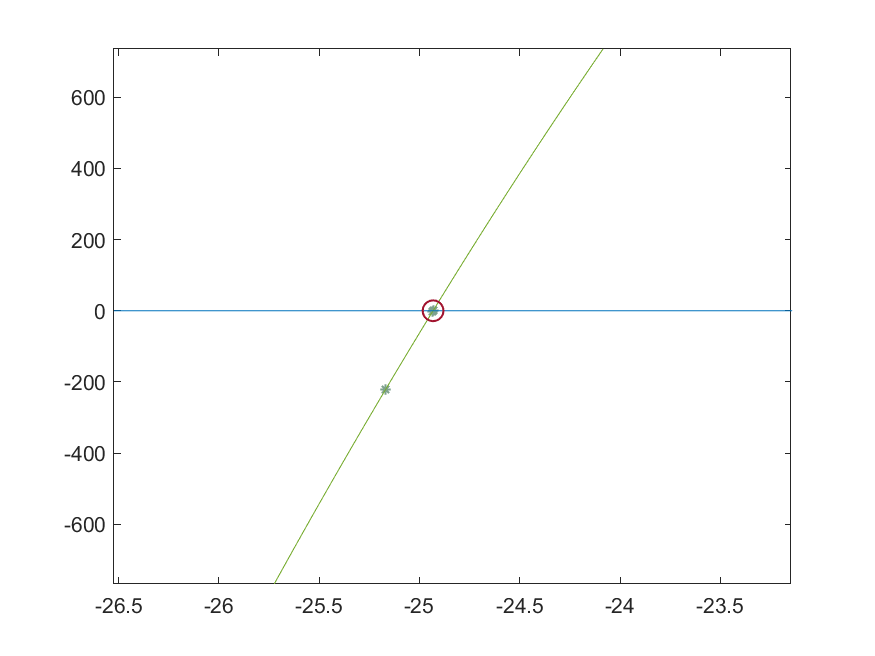
\includegraphics[width=9cm]{Images/coolFig.png}
        \caption{Gráfica resultante de \texttt{visualNewtonRoot}}
        \label{owo}
    \end{figure}

  \end{enumerate}

\newpage
\section{Anexos}

\texttt{newtonRoot.m}
\begin{lstlisting}
function output = newtonRoot(fun, der, ini, ite)
    if (isa(fun, 'function_handle') && isa(der, 'function_handle') && ite > 0)
        nextVal = ini;
        output = NaN;
        if(fun(nextVal) == 0) 
            disp(['Root found! ', num2str(nextVal), ' is the root for ', func2str(fun), '!'])
            output = nextVal;    
            return;
        else
            %% Skip %%
        end
        
        for index = 1:ite
            nextVal = nextVal - (fun(nextVal)/der(nextVal));
            
            if(fun(nextVal) == 0) 
                disp(['Root found! ', num2str(nextVal), ' is the root for ', func2str(fun), '!', ' Found after ', num2str(index), 'iterations'])
                output = nextVal;
                return;
            else
                %% Skip %%
            end
        end

        if abs(fun(nextVal)) < 10^(-5)
            output = nextVal;
            disp(['Approximate root found! ', num2str(nextVal)]);
        else
            disp('No roots found...')
        end

    else
        disp('Passed params are invalid!')
    end
end 
\end{lstlisting}
\texttt{newtonRunner.m}
\begin{lstlisting}
f = @(x) (x^3)+(13*(x^2))-(297.5*x)+(0.00000375*(exp(x)));
der = @(x) (3*(x^2))+(26*x)-(297.5)+(0.00000375*(exp(x)));
ite = 900;
ini = 12;
newtonRoot(f, der, ini, ite)
\end{lstlisting}
\texttt{modNewtonRoot.m}
\begin{lstlisting}
function output = modNewtonRoot(fun, der, ini, ite)
    if (isa(fun, 'function_handle') && isa(der, 'function_handle') && ite > 0)
        nextVal = ini;
        output = NaN;
        if(fun(nextVal) == 0) 
            disp(['Root found! ', num2str(nextVal), ' is the root for ', func2str(fun), '!'])
            output = nextVal;
            return;
        else
            %% Skip %%
        end
        
        for index = 1:ite
            lastVal = nextVal;
            nextVal = nextVal - (fun(nextVal)/der(nextVal));

            disp(['Realizando iteracion #', num2str(index)] )
            disp(['Raiz actual: ', num2str(nextVal)])
            disp(['f(', num2str(nextVal),') = ', num2str(fun(nextVal))])
            disp(['f''(', num2str(nextVal),') = ', num2str(der(nextVal))])
            disp(['Error absoluto = ', num2str(abs(nextVal-lastVal))])
            disp('-----------')
            
            if(fun(nextVal) == 0) 
                disp(['Root found! ', num2str(nextVal), ' is the root for ', func2str(fun), '!', ' Found after ', num2str(index), 'iterations'])
                output = nextVal;
                return;
            else
                %% Skip %%
            end
        end

        if abs(fun(nextVal)) < 10^(-5)
            output = nextVal;
            disp(['Approximate root found! ', num2str(nextVal)]);
        else
            disp('No roots found...')
        end

    else
        disp('Passed params are invalid!')
    end
end 
\end{lstlisting}
\texttt{moddedRunner.m}
\begin{lstlisting}
f = @(x) (x^3)+(13*(x^2))-(297.5*x)+(0.00000375*(exp(x)));
der = @(x) (3*(x^2))+(26*x)-(297.5)+(0.00000375*(exp(x)));
ite = 3;
ini = 1;
modNewtonRoot(f, der, ini, ite);
\end{lstlisting}
\texttt{visualNewtonRoot.m}
\begin{lstlisting}
function output = visualNewtonRoot(fun, der, ini, ite)
    if (isa(fun, 'function_handle') && isa(der, 'function_handle') && ite > 0)
        nextVal = ini;
        output = NaN;

        if(fun(nextVal) == 0) 
            disp(['Root found! ', num2str(nextVal), ' is the root for ', func2str(fun), '!'])
            output = nextVal;    
            return;
        else
            %% Skip %%
        end
        
        for index = 1:ite
            nextVal = nextVal - (fun(nextVal)/der(nextVal));

            plot(nextVal, fun(nextVal),'-*',...
            'LineWidth',1,...
            'MarkerSize',5,...
            'MarkerEdgeColor','#7EA28E')
            hold on

            if(fun(nextVal) == 0) 
                disp(['Root found! ', num2str(nextVal), ' is the root for ', func2str(fun), '!', ' Found after ', num2str(index), 'iterations'])
                output = nextVal;
                return;
            else
                %% Skip %%
            end
        end

        fplot(fun, [(nextVal - (fun(nextVal)/der(nextVal)))-1, (nextVal - (fun(nextVal)/der(nextVal)))+1])
        hold on

        line([nextVal-2 nextVal+2], [0 0])

        plot(nextVal, fun(nextVal),'-.ko',...
        'LineWidth',1,...
        'MarkerSize',10,...
        'MarkerEdgeColor','#A2142F')
        hold off

        if abs(fun(nextVal)) < 10^(-5)
            output = nextVal;
            disp(['Approximate root found! ', num2str(nextVal)]);
        else
            disp('No roots found...')
        end

    else
        disp('Passed params are invalid!')
    end
end     
\end{lstlisting}
\texttt{visualRunner.m}
\begin{lstlisting}
f = @(x) (x^3)+(13*(x^2))-(297.5*x)+(0.00000375*(exp(x)));
der = @(x) (3*(x^2))+(26*x)-(297.5)+(0.00000375*(exp(x)));
ite = 4;
ini = -27;
visualNewtonRoot(f, der, ini, ite);
\end{lstlisting}


\end{document}  


